\documentclass[11pt,reqno]{article}
\usepackage{amsmath,amssymb,mathrsfs,amsthm}
\usepackage[UTF8]{ctex}
%\usepackage{xeCJK}
%\setCJKmainfont{SimSum}

\usepackage{graphicx,cite,cases}
%\usepackage[pagewise]{lineno}\linenumbers
%\usepackage{refcheck}
\usepackage{xcolor}
\usepackage{bm}			% 公式加粗
\usepackage{tabularx}   % 绘制定宽表格
\usepackage{authblk}	% 添加更多作者信息
\usepackage{appendix} 	% 生成附录
\usepackage{listings}   % 附录里的代码, 支持语言高亮
\usepackage{hyperref}   % 超链接, 自动跳转
\hypersetup{	% 定义超链接效果
colorlinks=true,
linkcolor=blue,
anchorcolor=blue,
citecolor=blue}

\setlength{\topmargin}{-1.5cm}
\setlength{\oddsidemargin}{0.0cm}
\setlength{\evensidemargin}{0.0cm}
\setlength{\textwidth}{16.7cm}
\setlength{\textheight}{23cm}
\headheight 20pt
\headsep    26pt
\footskip 0.4in

%%%%% 关于公式编号问题 %%%%%
%统一用equation环境
%如果需要加括号用\begin{cases}
%如果公式过长需要分行用\begin{split}
%如果一个equation里面需要多个公式, emmm没研究过

\newtheorem{theorem}{Theorem}[section]
\newtheorem{corollary}[theorem]{Corollary}
\newtheorem{lemma}[theorem]{Lemma}
\newtheorem{proposition}[theorem]{Proposition}
\newtheorem{remark}[theorem]{Remark}
\newtheorem{definition}[theorem]{Definition}
\numberwithin{equation}{section}


\renewcommand{\d}{\,\mathrm d}
\usepackage{algorithm,algorithmicx}  %写伪代码
\usepackage{algpseudocode}			% 写伪代码
%%%%%% 算法部分改为中文显示 %%%%%%%%%
%%\floatname{algorithm}{算法}
\renewcommand{\algorithmicrequire}{\textbf{Input:}}
\renewcommand{\algorithmicensure}{\textbf{Output:}}

%% Ctrl+Alt+R 编译
%% Ctrl+Alt+V 打开文档

\begin{document}

\title{微分方程数值解计算实习}

\author{朱荃凡}
\affil{(吉林大学数学系计算唐班)}
\date{\today}

\maketitle


\section{问题重述}

以下列两点边值问题为例
\begin{equation}
	\left\{
	\begin{aligned}
		& u''+u=-x,\ 0<x<1,\\
		& u(0)=u(1)=0.
	\end{aligned}
	\right.
	\end{equation}
取基函数为
\[\phi_i(x)=\sin(i\pi x),\quad\psi_i(x)=(1-x)x^i,\ i=1,2,\cdots,N.\]

1\ 对比两组基函数对应的系数矩阵的条件数随N增加产生的变化.

2\ 画图对比两组基函数对应的数值解与精确解
\begin{equation}
	u_*(x)=\frac{\sin x}{\sin 1}-x
\end{equation}
之间的$L^2([0,1])$误差随着N增加产生的变化.


\section{系数矩阵与条件数}

我们分别取两组基函数的个数k为1到8,计算出系数矩阵的条件数并列出如下表格:
\begin{table}[h]\label{table1}
	\begin{center}
	\caption{\zihao{5}{稀疏矩阵的条件数}}
	\begin{tabular}{|c|c|c|c|c|c|c|c|c|}
		\hline	
		 $k$ & 1 & 2 & 3 & 4 & 5 & 6 & 7 & 8\\
		\hline
		Cond1 & 1 & 4.34 & 9.90 & 17.69 & 27.71 & 39.95 & 54.41 & 71.10 \\
		\hline
		Cond2 &$1$ & $10.17$& $1.61\times10^2$ & $3.11\times10^3$ & $6.69\times10^4$
		& $1.55\times10^6$ & $3.80\times10^7$ & $9.66\times10^8$ \\
		\hline
	\end{tabular}
	\end{center}
\end{table}

从表中可以看出, 第一组基函数对应系数矩阵的条件数增长速度相当缓慢,介于线性和二次函数之间;而
多项式基函数对应系数矩阵的条件数呈现出指数级增长速度.这种现象可以从系数矩阵的结构解释,第一类系数矩阵是对角阵,
而第二类系数矩阵是一个无规律可循的满矩阵.



\section{误差收敛速度}

为计算数值解和真解之间的误差收敛速度,我们计算它们之间的$L^2$范数,即:
\begin{equation}
err_n=\left[\int_{0}^{1}(u_*(x)-u_n(x))^2\d x\right]^{1/2}.
\end{equation}
并且积分也是通过数值方法去实现的.具体来说,在$[0,1]$区间上等分取101个节点,计算这些
节点处的真解和数值解的数值,然后使用复化Simpson公式.最后我们绘制出如下的误差收敛图:

\begin{figure}[h]
	\begin{center}
		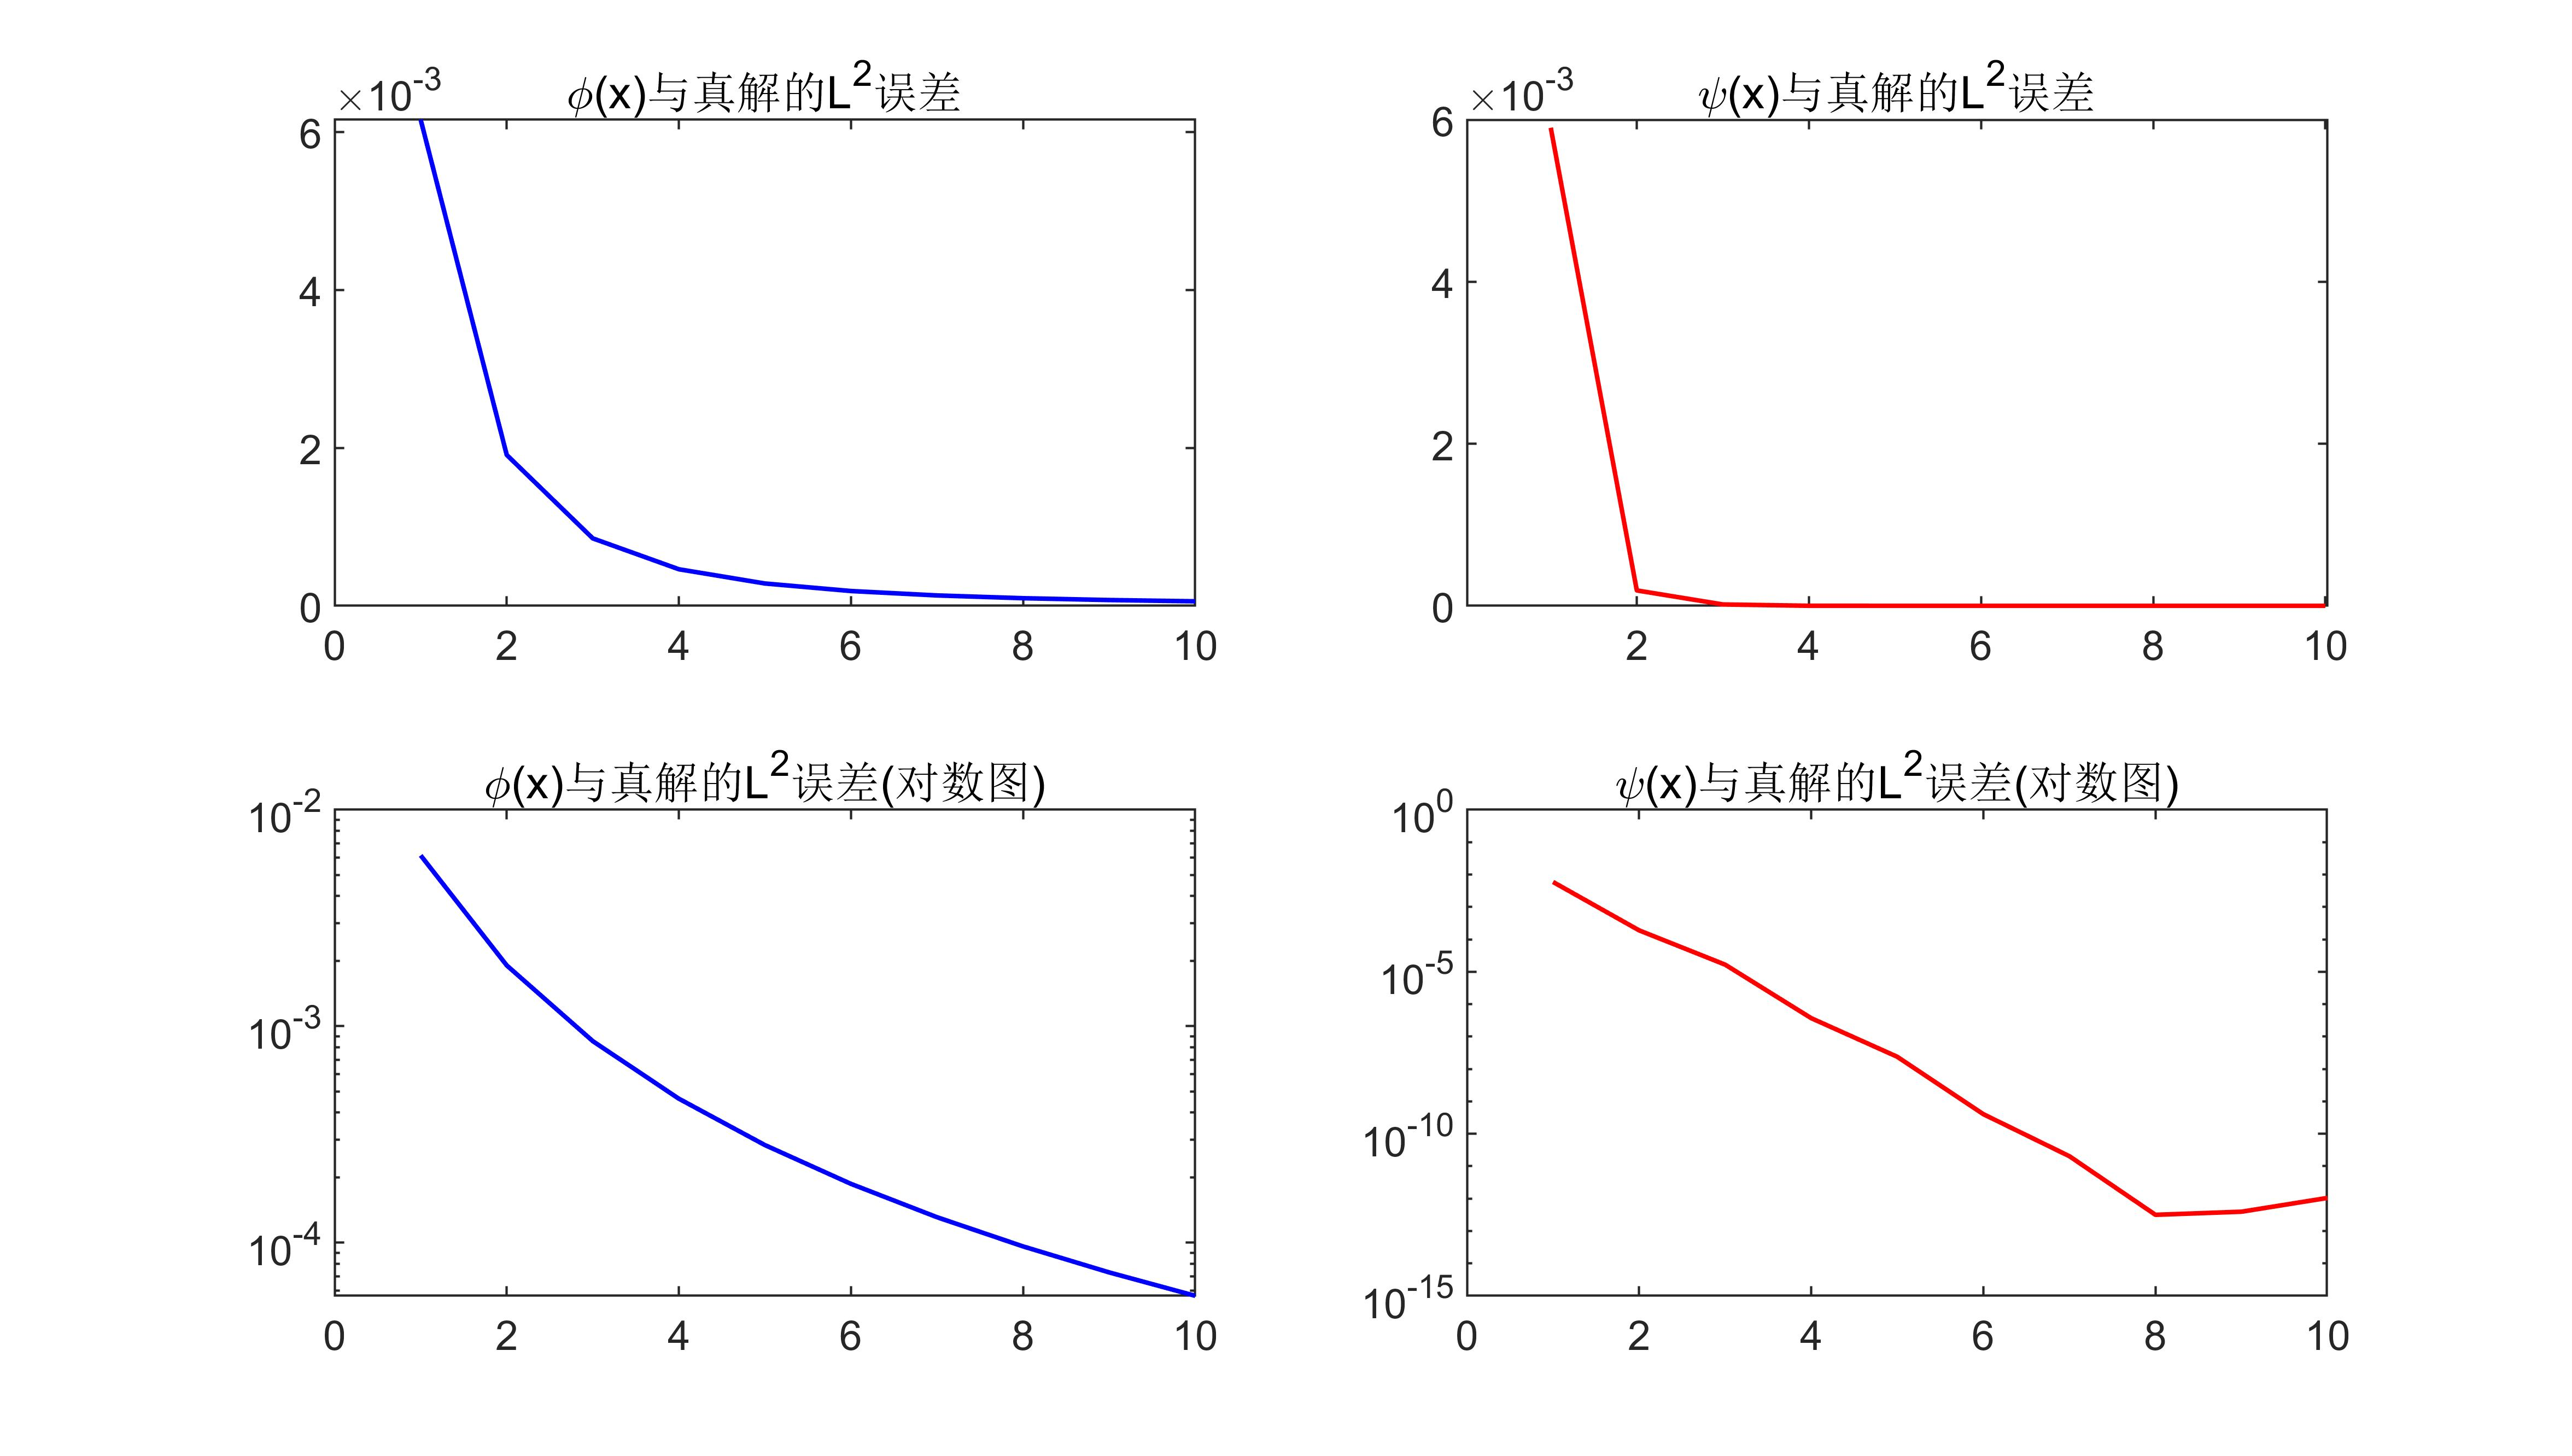
\includegraphics[width=1\textwidth]{pic3.jpg}
	\end{center}
\end{figure}

从图中可以看出,三角基函数和多项式基函数得到的数值解与真解之间的$L^2$误差均有指数级
的收敛速度, 并且多项式类收敛更快,在对数图中,当$k\ge9$时甚至出现了运算精度造成的结果错误.
综上,基函数的选取对Ritz-Galerkin方法的收敛速度十分重要.



\end{document}
